\documentclass[twocolumn, 12pt]{article}

\usepackage[utf8]{inputenc}
\usepackage[english, spanish]{babel}
\usepackage{fullpage} % changes the margin
\usepackage{graphicx}
\usepackage{amsmath}
\usepackage{enumitem}
\usepackage{chngcntr}
\usepackage{setspace}
\usepackage{url}
\usepackage{csquotes}
\usepackage{float}
\usepackage{verbatim}
\usepackage{tabularx}
\usepackage{amsmath}

\counterwithin{figure}{section}
\renewcommand{\thesection}{\arabic{section}}
\renewcommand{\thesubsection}{\thesection.\arabic{subsection}}
\renewcommand{\baselinestretch}{1.5}

\usepackage[style=apa, maxnames=6, minnames=3, backend=biber]{biblatex}
\DefineBibliographyStrings{english}{%chktex-file 1 chktex-file 6
	andothers = {\em et\addabbrvspace al\adddot}
}
\addbibresource{./Bibliography/bibliography.bib}

\usepackage{array}
\usepackage{enumitem}
\usepackage{floatrow}

\raggedbottom{}

\begin{document}

\begin{titlepage}
	\centering
	
\includegraphics[width=0.3\textwidth]{Images/logo_utb.png}\par\vspace{1cm}
	{\scshape\LARGE Universidad Tecnológica de Bolívar \par}
	\vspace{1cm}

	{\scshape\Large FÍSICA ELÉCTRICA \par}
	\vspace{.2cm}

	% chktex-file 8
	{\scshape\Large H1 - C \par}
	\vspace{1cm}
	% chktex-file 8
	\slshape {\Large \bfseries{}Informe de Laboratorio No. VI\\}
	\vspace{1cm}

	\slshape {\itshape{} Mauro González, T00067622 \\}
	\slshape {\itshape{} German De Armas Castaño, T00068765 \\}
	\slshape {\itshape{} Angel Vega Rodriguez, T00068186 \\}
	\slshape {\itshape{} Juan Jose Osorio Ariza, T00067316 \\}
	\slshape {\itshape{} Juan Eduardo barón, T00065901 \\}
	\vfill
	Revisado Por \\
	Gabriel Hoyos Gomez Casseres\\
	{\large \today\par}
\end{titlepage}

% ----------------------------------------------------------------------|>
\section{Introducción}

Los fenómenos electromagnéticos son aquellos que se
producen como resultado de la interacción entre campos
eléctricos y magnéticos, los cuales se asocian a la
presencia de cargas eléctricas en movimiento.

En el desarrollo de esta practica se busca comprender a
profundidad distintos fenómenos electromagnéticos
justificados con distintos postulados dados a partir de
famosas leyes como la ley de Faraday, Lenz y maxwell.

Además de establecer relaciones lógicas entre los conceptos
de campo eléctrico y magnético analizando sus interacciones
y comportamientos tanto de forma individual como en
conjunto, todo apoyado de apreciaciones experimentales que
serán divulgadas a lo largo del informe.

% ----------------------------------------------------------------------|>
\section{Objetivos}

\subsection*{Objetivo general}

\begin{itemize}[label=$\triangleright$]
	\item Visualizar y explicar los fenómenos donde se evidencia la
	      relación entre campo eléctrico y campo magnético
\end{itemize}

\subsection*{Objetivos específicos}

\begin{itemize}[label=$\triangleright$]
	\item Explicar como funciona cada fenómeno electromagnético a
	      partir de las leyes formuladas
	\item Entender los principios físicos detrás de los aparatos como
	      transformadores,bobinas o incluso brújulas, analizando como
	      varían dependiendo su corriente.
	\item Analizar el principio de inducción tomando como referencia
	      lo establecido por la ley de Faraday y Lenz
\end{itemize}

% ----------------------------------------------------------------------|>
\section{Marco Teórico}

% ----------------------------------------------|>
\subsection*{Ley de Faraday}

Establece que un cambio en el flujo magnético a través de
una superficie cerrada induce una fuerza electromotriz
\textit{(FEM)} en un circuito eléctrico que rodea esa
superficie. De ahí que se conozca que la tensión inducida
en un circuito cerrado es directamente proporcional a la
rapidez del cambio de flujo magnético que pasa a través de
una espira (o lazo). Matemáticamente, la ley de Faraday se
expresa como:

{\Huge
\begin{equation}
	\varepsilon = - \frac{d \phi_B}{dt}
\end{equation}
}

El signo menos es una indicación del sentido de la
\textit{FEM} inducida. Si la bobina tiene N vueltas,
aparece una fem en cada vuelta que se pueden sumar, es el
caso de los tiroides y solenoides, en estos casos la fem
inducida será:

{\large
\begin{equation}
	\varepsilon = - N \frac{d \phi_B}{dt} = - \frac{d (N \phi_B)}{dt}
\end{equation}
}

Fuente:~\cite{CorderoElectromagnetismo}

% ----------------------------------------------|>
\subsection*{Ley de Lenz}

Es una consecuencia del principio de conservación de la
energía aplicado a la inducción electromagnética la cual
nos dice en qué dirección fluye la corriente, y establece
la dirección de la corriente inducida debe ser tal que su
propio campo magnético se dirija de una manera que se
oponga al flujo cambiante que causa el campo del imán que
se aproxima, es decir, la dirección siempre es tal que se
opone al cambio de flujo que la produce. Esto significa que
cada campo magnético generado por una corriente inducida va
en la dirección opuesta al cambio en el campo original.

Por lo tanto, la corriente inducida circula de manera que
sus líneas de campo magnético a través del bucle se dirigen
desde la parte trasera a la delantera del bucle.

	{\Large
		\begin{equation}
			\varepsilon = - \frac{d \phi}{dt}
		\end{equation}
	}

% ----------------------------------------------|>
\subsection*{Ley de Apere y ley de Ampere-Maxwell}

La ley de Ampere establece que un campo magnético que pasa
por una trayectoria cerrada por el que fluye la corriente,
provoca que este campo magnético sea igual a la
permeabilidad constante del espacio, multiplicada por la
fuerza total de la corriente. En otras palabras, la ley
establece que la corriente que fluye en un conductor
produce un campo magnético. La ley de los amperios de
Maxwell establece que un campo magnético que pasa por un
camino cerrado que contiene una corriente hace que este
campo magnético sea igual a la permeabilidad constante del
espacio igual a la suma de los dos tipos de corrientes;
corriente total y corriente de desplazamiento. En otras
palabras, la ley establece que los campos magnéticos son
producidos tanto por corrientes de conducción como de
desplazamiento.

Esta ley determina que la circulación del campo magnético a
lo largo de una línea cerrada es equivalente a la suma
algebraica de las intensidades de las corrientes que
atraviesan la superficie delimitada por la línea cerrada,
multiplicada por la permitividad del medio. En concreto
para el vacío:

{\Large
\begin{equation}
	\oint \vec{B} d\vec{l} = \mu_0 I_T
\end{equation}
}

Fuente:~\cite{LeyesMaxwell}

% ----------------------------------------------|>
\subsection*{Corrientes parasitas}

Las corrientes parasitas, también conocidas como corrientes
de Foucault, son corrientes eléctricas que se producen en
un material conductor cuando se encuentra en presencia de
un campo magnético variable. Estas corrientes son inducidas
por la variación del campo magnético y circulan en el
material conductor, lo que puede provocar efectos no
deseados en algunos dispositivos
eléctricos~(\cite{reyes_pinto_2014}).

% ----------------------------------------------|>
\subsection*{Transformador}

Es una máquina eléctrica que, basándose en los principios
de inducción electromagnética, transfiere energía de un
circuito eléctrico a otro, sin cambiar la frecuencia. La
transferencia se lleva a cabo con el cambio de voltaje y
corriente. Un transformador aumenta o disminuye la
corriente alterna cuando es necesario.

Estas máquinas ayudan a mejorar la seguridad y eficiencia
de los sistemas de energía durante su distribución y
regulación a través de largas
distancias~(\cite{tecsa_2021})

El principio de funcionamiento del transformador se basa en
la ley de Faraday de la inducción electromagnética. Cuando
se aplica una corriente alterna a la bobina primaria del
transformador, se produce un campo magnético que induce una
corriente eléctrica en la bobina secundaria.

La relación entre el número de vueltas de la bobina
primaria y secundaria determina la relación de voltaje
entre las dos bobinas~(\cite{rodriguez_2014})

% ----------------------------------------------------------------------|>
\section{Montaje experimental y análisis de datos}

% ---------------------------------------------------|>
\subsection*{Experimento 1 - Inducción electromagnética}

Para este primer experimento se cuenta con una bobina
conectada a un galvanómetro, un imán y una brújula. Cuando
se introduce el imán a la bobina, se crea una corriente
eléctrica que alimenta a la misma, y como hay corriente
eléctrica, se crea un campo magnético. Este ultimo influye
en el movimiento de la aguja del galvanómetro que oscila en
los extremos de forma continua debido al tipo de corriente
inducida. Si fuera con corriente continua (DC), la aguja
del galvanómetro se desviaría hacia un lado o hacia el otro
en función de la dirección de la corriente que lo
atraviesa. En cambio, en corriente alterna (AC), la
corriente cambia de dirección constantemente, generando
esta oscilación en la aguja. Este experimento busca
demostrar la Ley de inducción electromagnética de Faraday y
la Ley de Lenz.

\begin{figure}[H]
	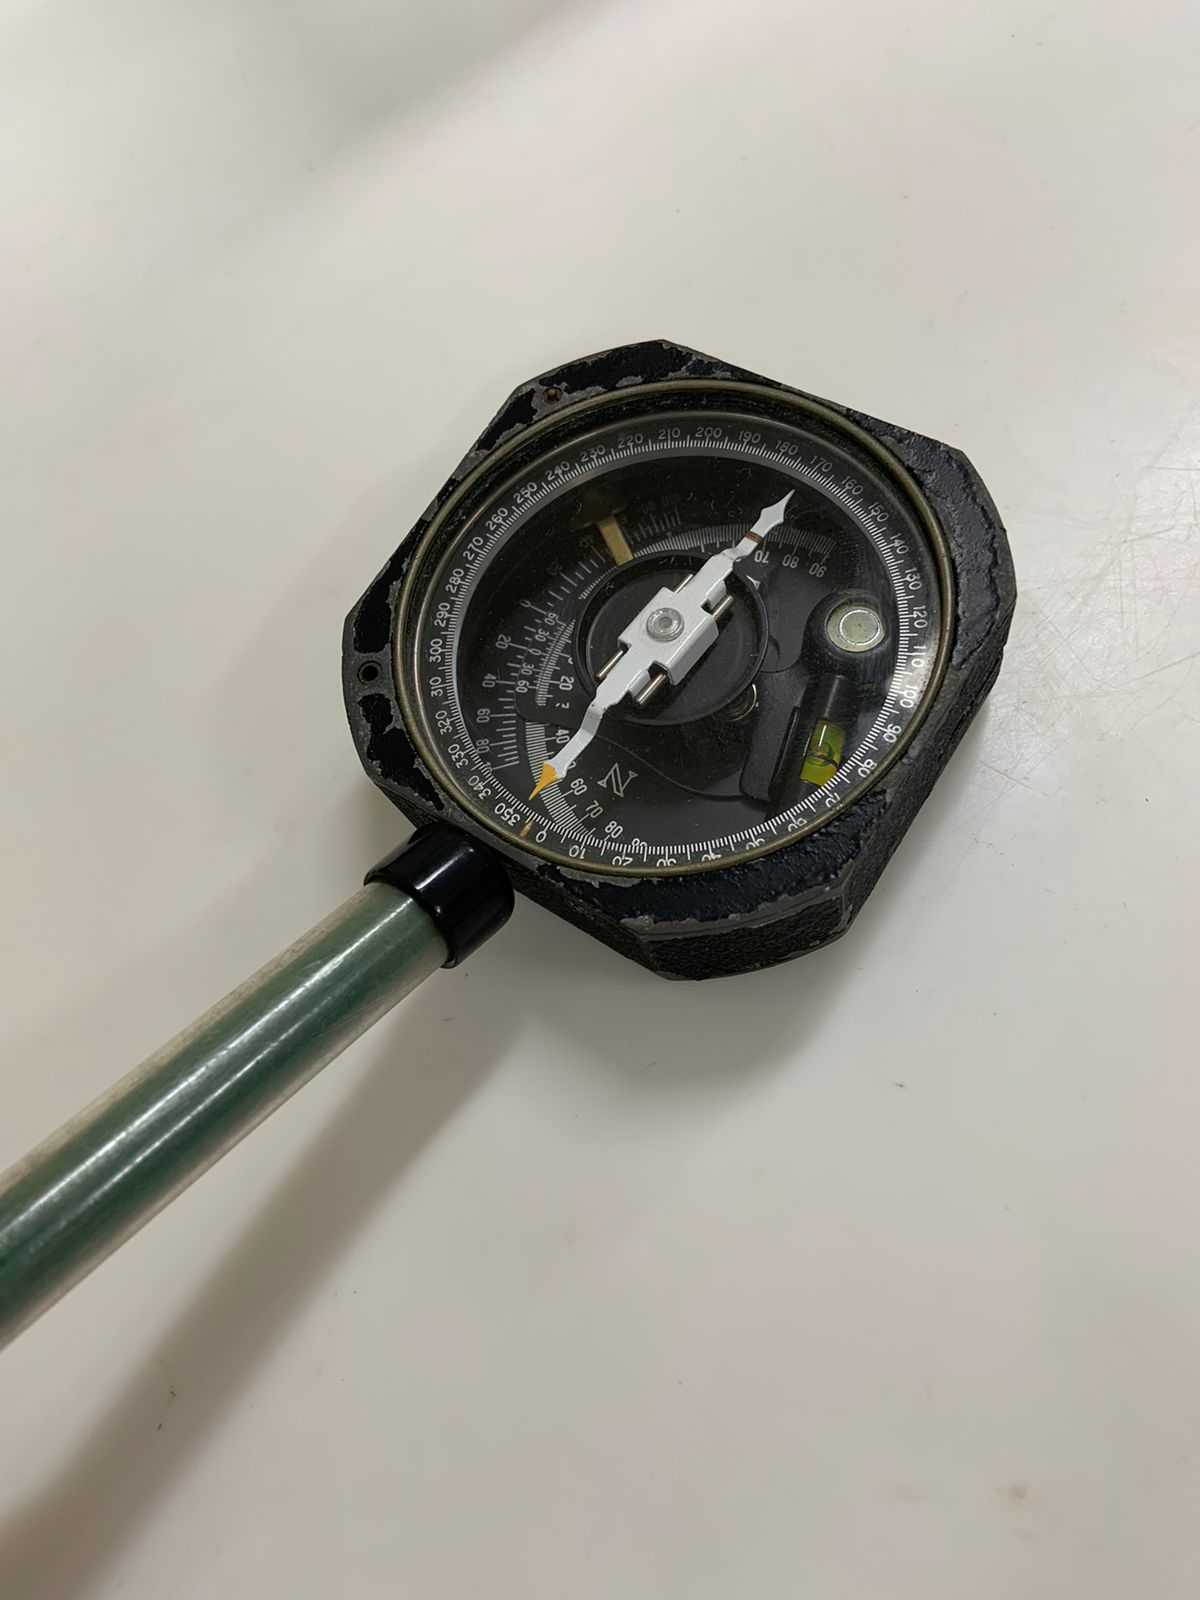
\includegraphics[width=0.9\linewidth]{./Images/BrujulaImagen1.jpeg}
\end{figure}

\begin{figure}[H]
	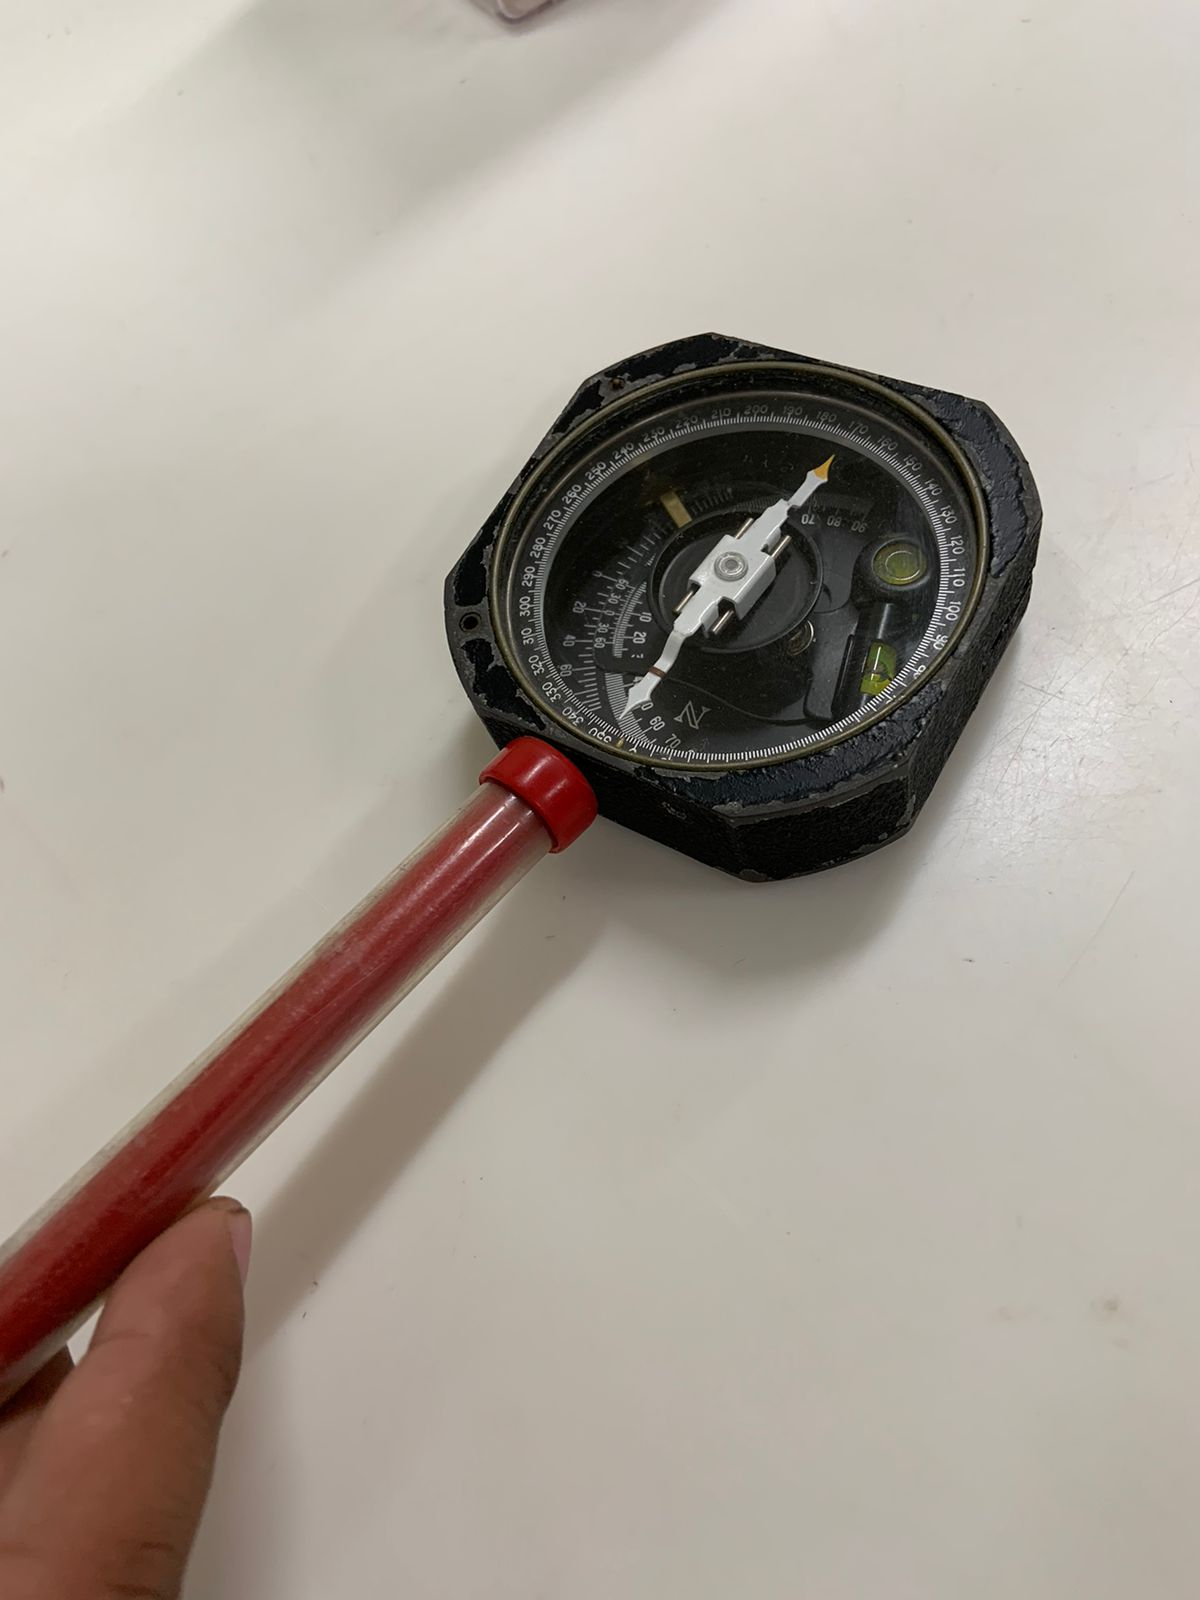
\includegraphics[width=0.9\linewidth]{./Images/BrujulaImagen2.jpeg}
\end{figure}

\begin{figure}[H]
	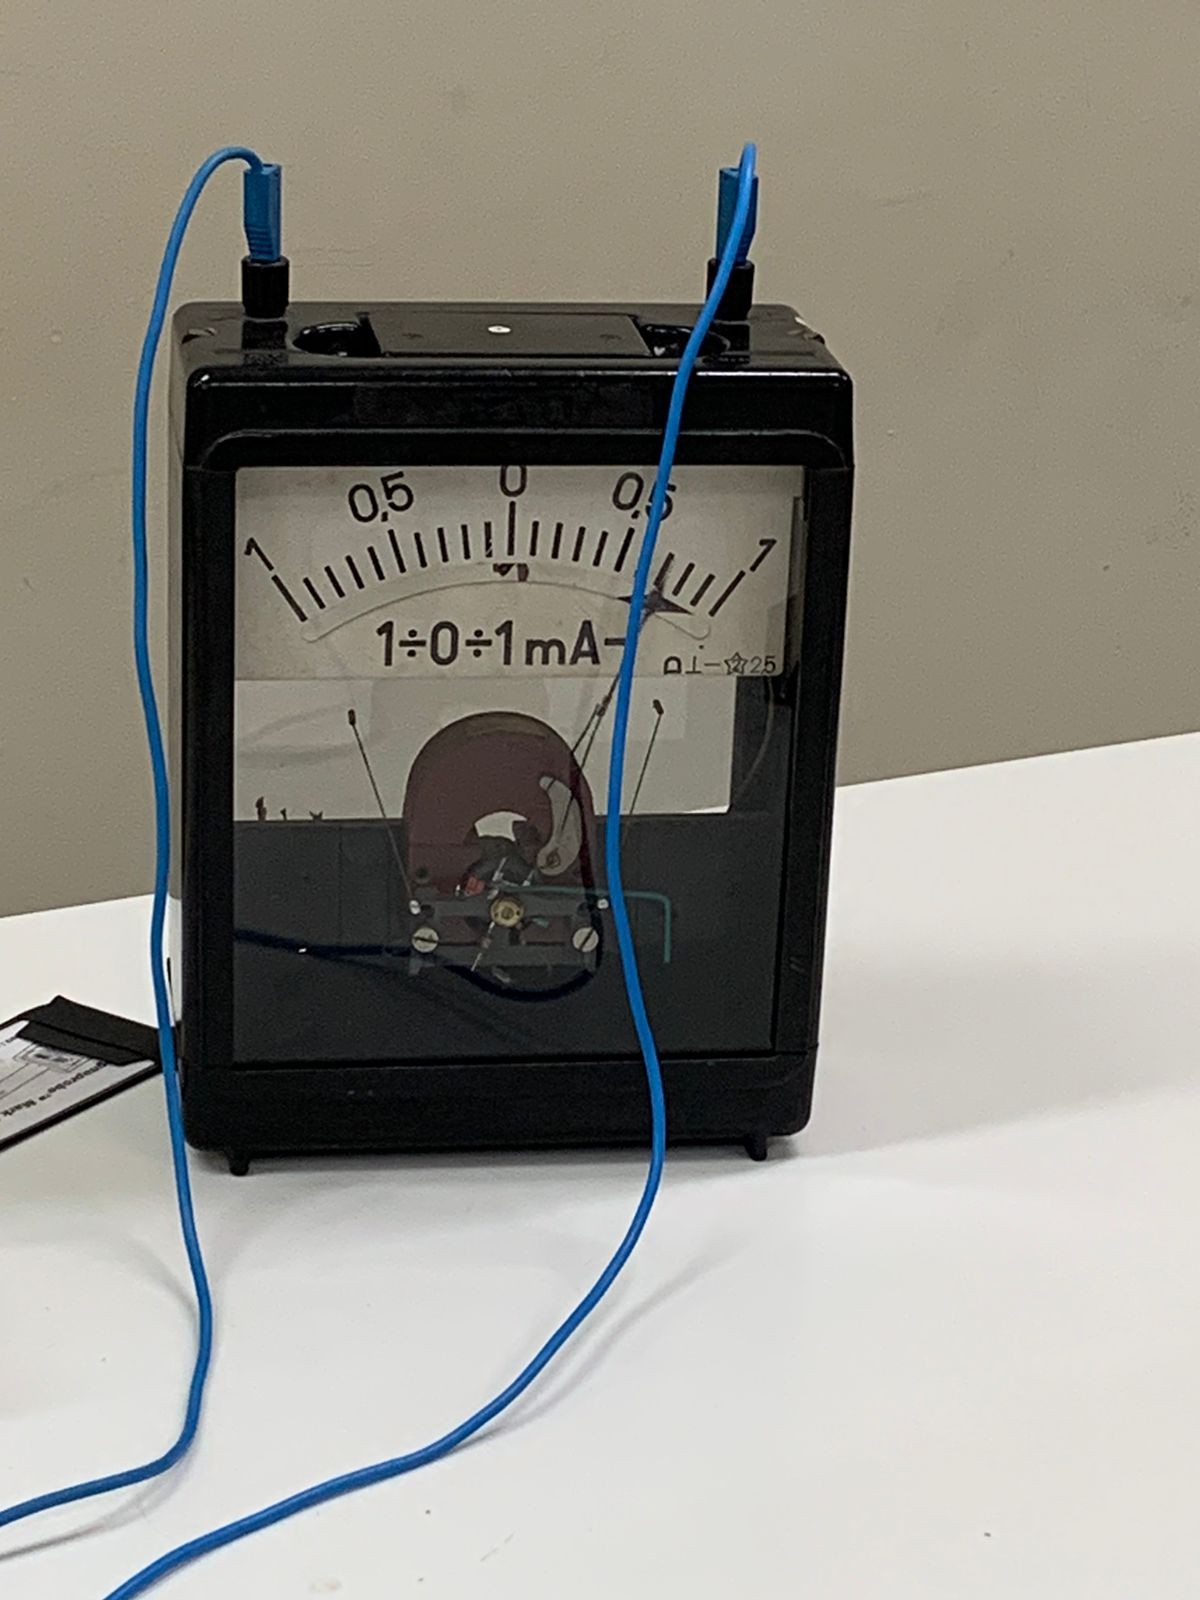
\includegraphics[width=0.9\linewidth]{./Images/Galvanometro1.jpeg}
\end{figure}

\begin{figure}[H]
	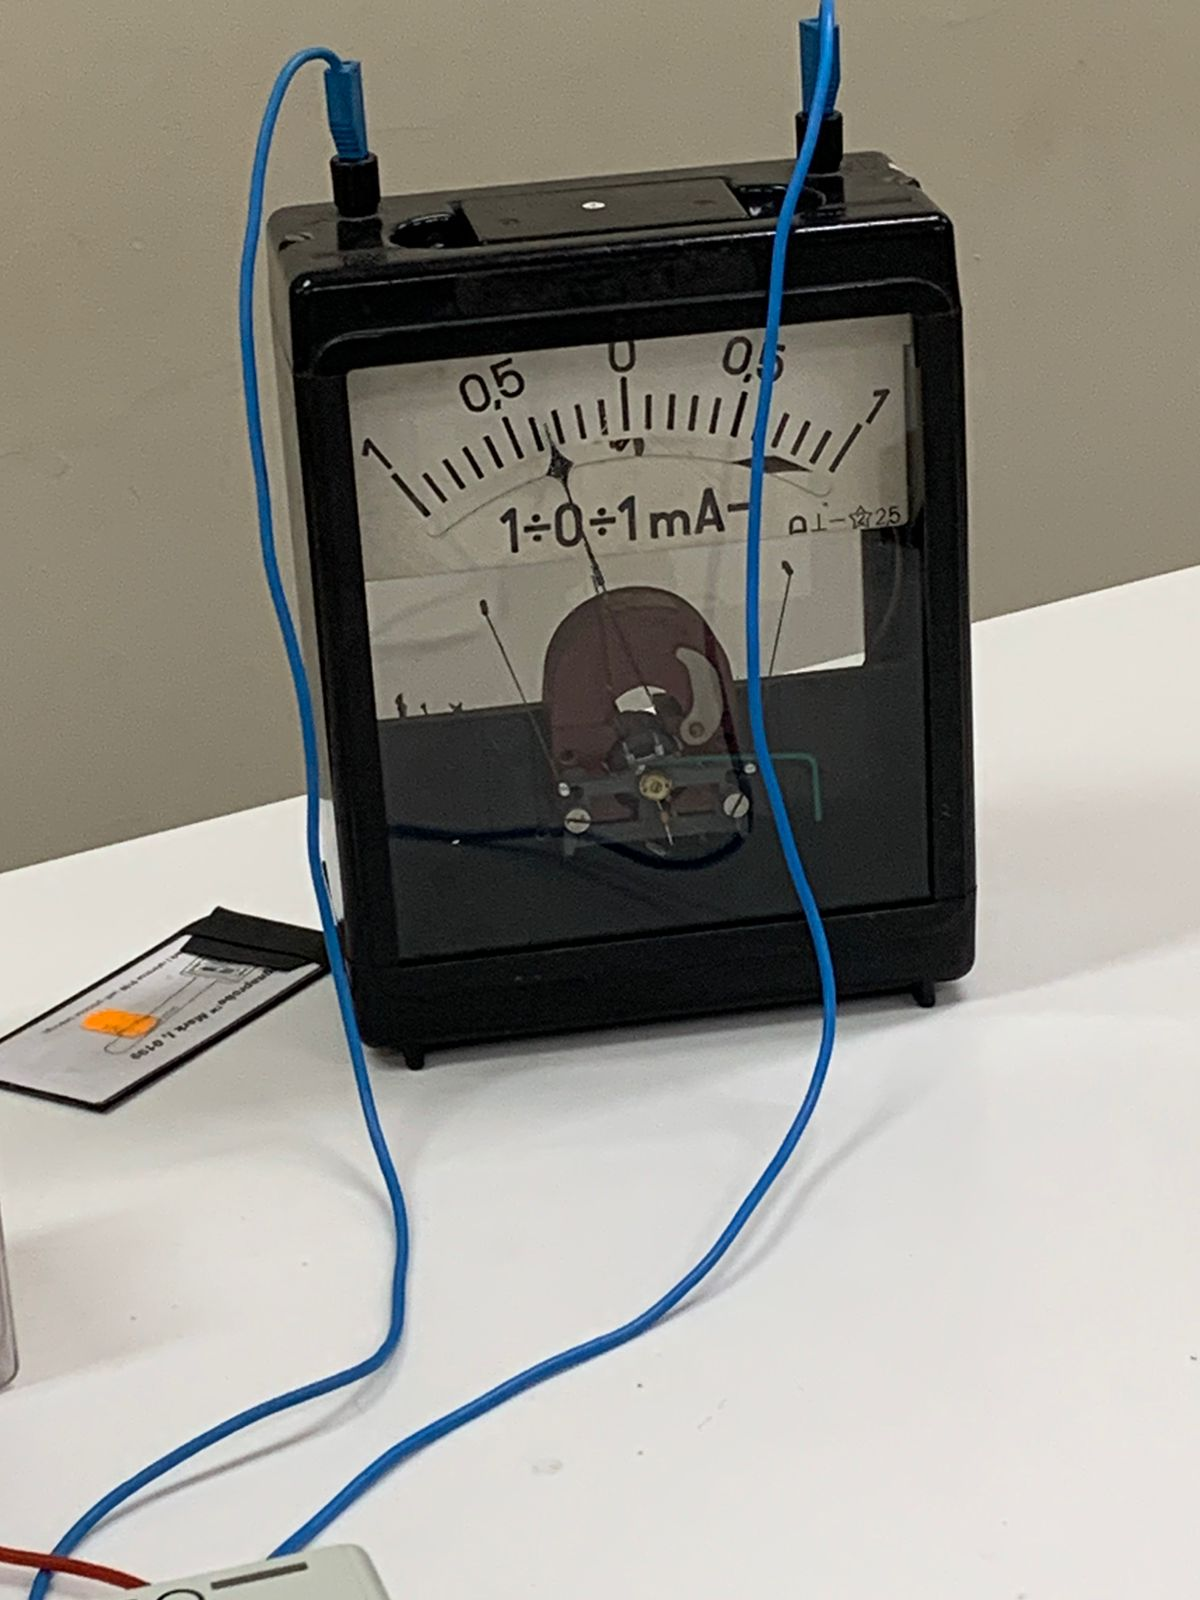
\includegraphics[width=0.9\linewidth]{./Images/Galvanometro2.jpeg}
\end{figure}

% ---------------------------------------------------|>
\subsection*{Experimento 2 - Transformador con corriente directa}

En este experimento se utiliza un electroimán (de núcleo de
hierro), una fuente de corriente directa, una bobina y un
galvanómetro. El electroimán se conecta a una fuente de
poder y se enciende y apaga intermitentemente para crear un
flujo de corriente eléctrica en la bobina, y se conectan
las terminales de la bobina al galvanómetro. Cuando a la
bobina se le induce corriente se crea un flujo de campo
magnético alrededor, que atrae a los materiales metálicos
cercanos. Otras observaciones destacables sobre la
estructura del experimento son: la fuente de poder no tiene
contacto con la bobina; solo se genera corriente eléctrica
al encender y apagar de forma intermitentemente la fuente
de poder.

\begin{figure}[H]
	\includegraphics*[width=0.9\linewidth]{./Images/Electroiman.jpeg}
\end{figure}

\begin{figure}[H]
	\includegraphics*[width=0.9\linewidth]{./Images/Electroiman2.jpeg}
\end{figure}

% ---------------------------------------------------|>
\subsection*{Experimento 3 - Transformador con corriente alterna}

Para este experimento de física, necesita hacer un
transformador experimental con dos bobinas (una primaria y
una secundaria unidas a un núcleo de hierro en forma de u),
un toma corriente, un interruptor y dos voltímetros. Cuando
se aplica corriente alterna a la bobina primaria, se crea
un flujo magnético alrededor de las bobinas. Cuando se
colocan ambas bobinas sobre el núcleo de hierro en u y se
pasa corriente, se crea un flujo magnético alrededor del
núcleo y dentro de la bobina secundaria se crea una tensión
alterna. Durante el experimento, se observa cómo hay una
pérdida de voltaje debido a unos orificios en la parte
superior del núcleo. Esta pérdida se debe a que el flujo
magnético se pierde al no estar completamente cerrado en el
circuito, por lo que se prueban distintos materiales de
diferente área y masa para completar el circuito. La
pérdida de voltaje se debe a varios factores: el número de
vueltas de la bobina secundaria en el núcleo, debido a que
la corriente es directamente proporcional a dicho número;
que el circuito no esté completamente cerrado en el núcleo,
puesto que se da una fuga, y no se puede aprovechar al
máximo la corriente inducida.

\begin{figure}[H]
	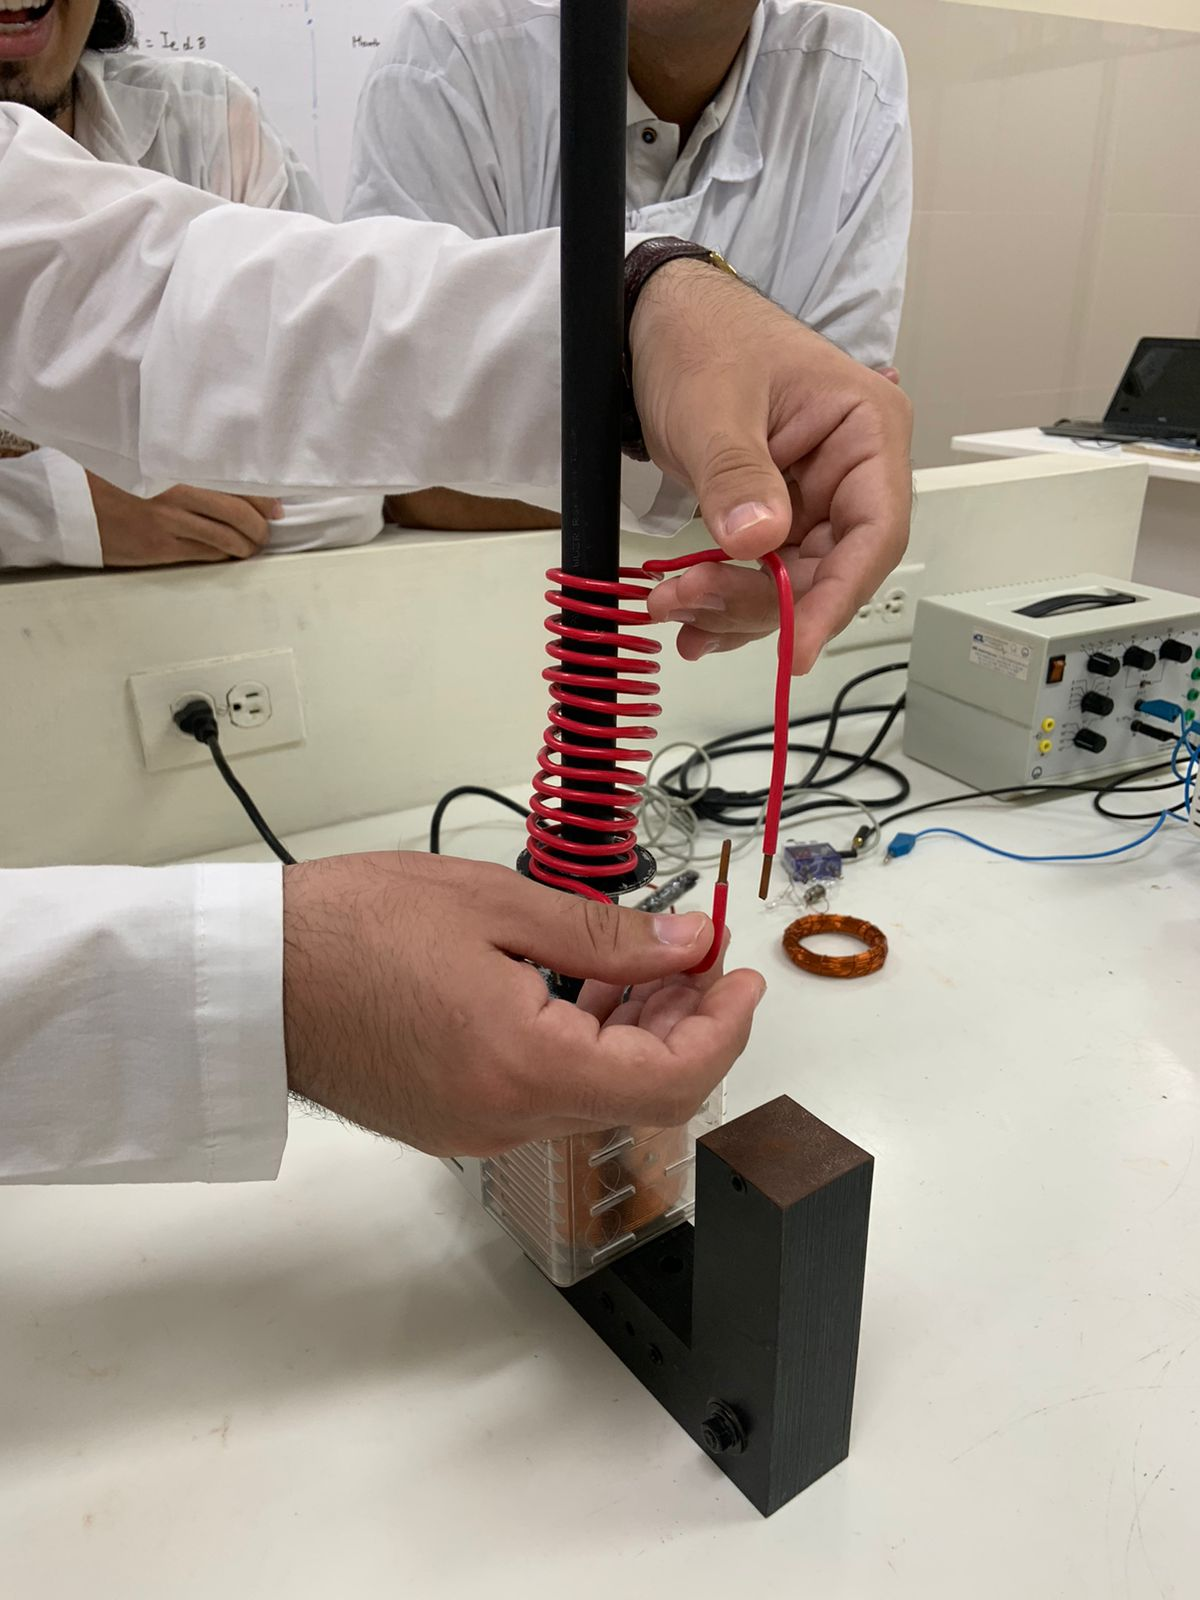
\includegraphics[width=0.9\linewidth]{./Images/DIFPotencial.jpeg}
\end{figure}

% ---------------------------------------------------|>
\subsection*{Experimento 4 - Inducción electromagnética y corrientes parasitas}

Para este experimento se utilizan dos anillos de aluminio
(uno con una ranura), una bobina conectada a varios
bombillos, un núcleo de hierro y una resistencia eléctrica
o reóstato. Se conecta la resistencia a la bobina y se
coloca una barra de hierro encima. A medida que se acerca
más la bobina con los bombillos al núcleo, la bombilla
alumbra con mayor intensidad. Ahora bien, cuando se
introduce el anillo de aluminio, éste sale disparado en
dirección contraria debido a que cuando ingresa la
corriente alterna a la bobina se generan polos y flujo
magnético en la bobina y en el tubo de hierro, lo cual
induce en el anillo una intensidad de corriente y polos
magnéticos, por lo tanto, cuando llega la corriente, los
polos son iguales y por esto sale disparado el anillo.
Ahora bien, cuando se aumenta la resistencia, el anillo
levita porque los flujos magnéticos no son suficientes para
vencer el peso del anillo. Si el anillo presenta fisuras,
éste no experimentará ningún fenómeno de magnetismo, aunque
en esencia todos los anillos sean iguales debido a que las
fisuras interrumpen la continuidad de la conductividad
eléctrica y magnética.

\begin{figure}[H]
	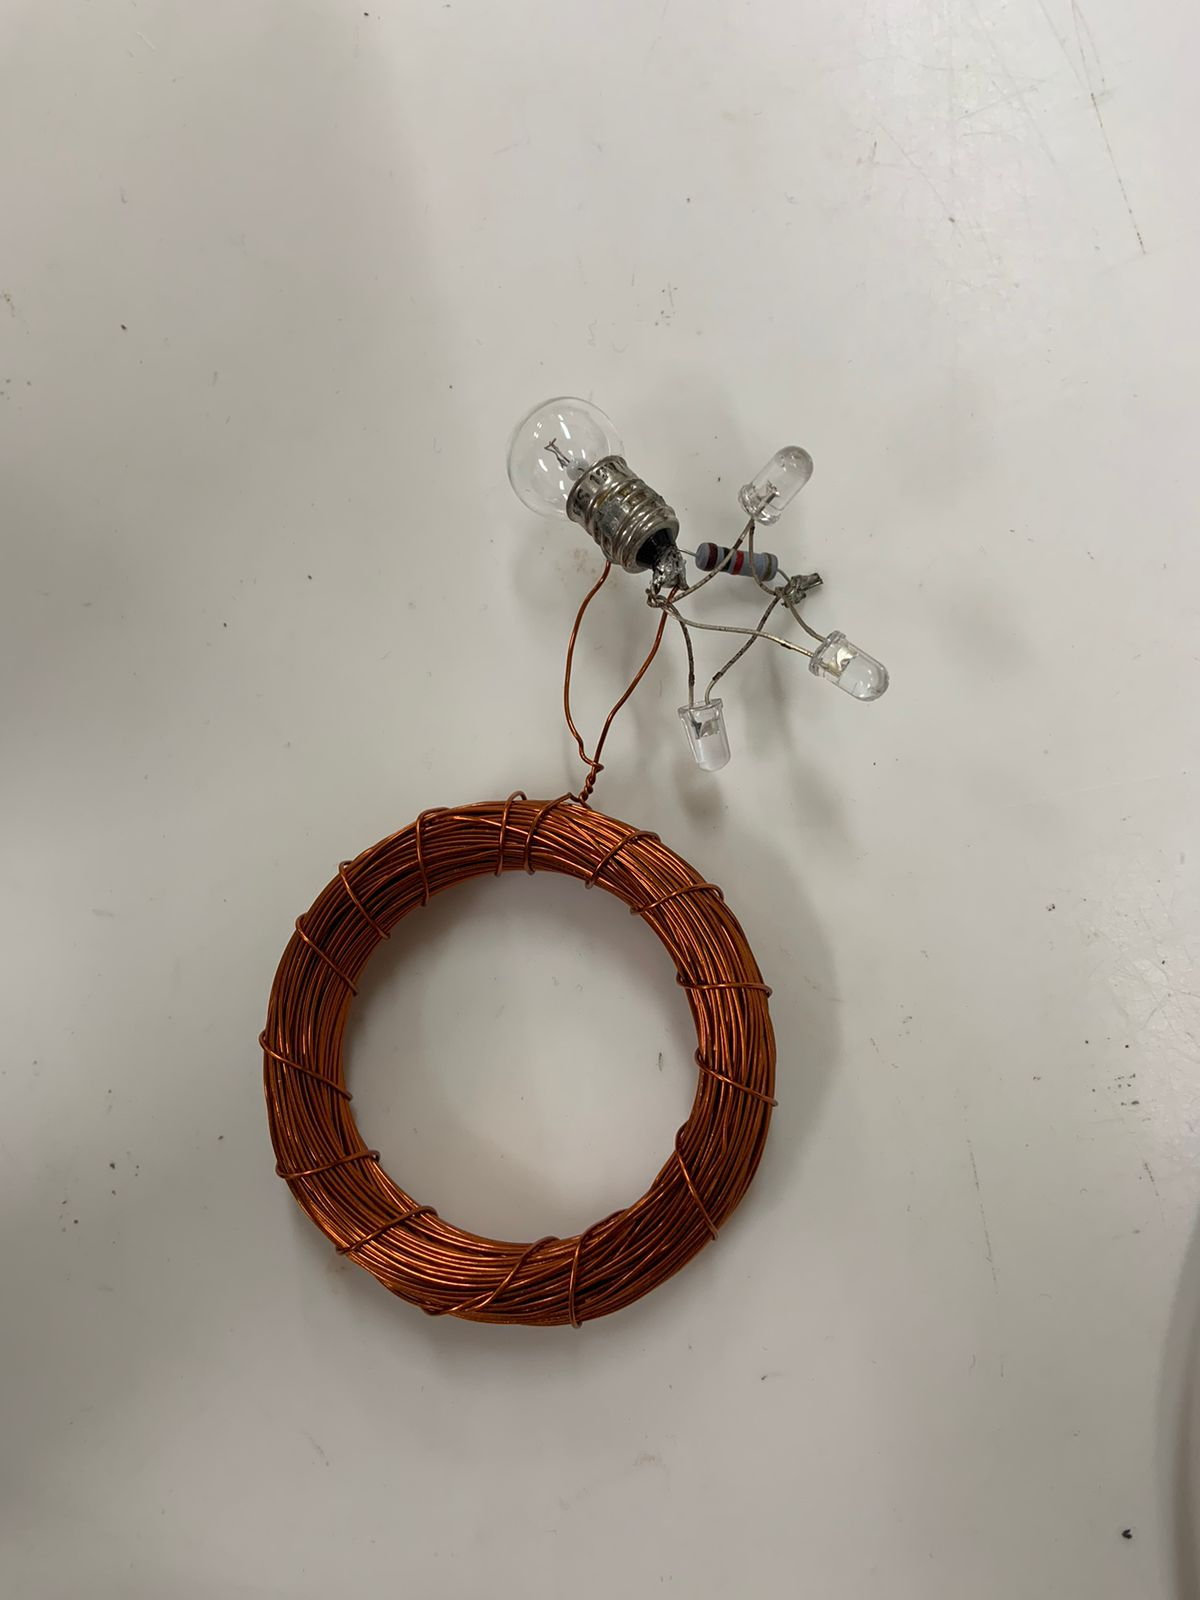
\includegraphics[width=0.9\linewidth]{./Images/Foquito.jpeg}
\end{figure}

% ----------------------------------------------------------------------|>
\section{Conclusiones}

En la anterior experiencia se abordaron leyes que nos
ayudan a comprender de mejor manera algunos fenómenos
electromagnéticos y a su vez permite evidenciar la relación
entre campo eléctrico y campo magnético desde la teoría en
la que se explica la interacción que poseen dos cuerpos
cuando son cargados de alguna u otra forma, hasta la
importancia que conlleva esto en la experimentación y
utilidad tanto en la explicación de fenómenos como en la
implementación en los dispositivos a lo largo de los
tiempos como lo fue la brújula. El conocimiento de los
fenómenos electromagnéticos ha contribuido en gran medida
en el desarrollo de la tecnología, facilitando su creación
y contribuyendo de forma segura a su constante uso en la
actualidad.

\printbibliography

\end{document}